\section{Stromrichter}
Die Leistungselektronik wir in einem mobilen Container, der für die Außenaufstellung ausgelegt wird untergebracht und verbindet die beiden Transformatoren.
Die Zwischenkreiskomponenten wie die Drosseln, Kondensatoren und Widerstände werden ebenfalls außen aufgestellt und mit dem COntainer verbuden. 

\subsection{Allgemeine Merkmale}
\begin{table}[htb]
    \centering
    \begin{NiceTabular}{|l|c|}[]
        \CodeBefore
        \columncolor{lightergray}{1}
        \Body
        \hline
         Aufstellung & Container(Innenraum)\\
         \hline
         Verschmutzung & Verschmutzungsgrad II (normal) \\
         \hline
         Aufstellungshöhe & < 1000 m üNN\\
         \hline
         Umgebungstemperatur &  -30°C bis 40°C\\
         \hline
         Klimabedingungen & Normal\\ 
         \hline
                 \Block{3-1}{Dokumentationen} &  \tabitem Technische Zeichnungen und CAD\\
                         &\tabitem Montageplan, Wartungsplan, Dokumentationen\\
                         &\tabitem Prüfprotokoll der zu erfüllenden Prüfungen\\
            \hline
    \end{NiceTabular}
\end{table}
\subsubsection*{Halbleiter IGBT 4,5kv 4kA}
\begin{itemize}
    \item Leistungshalbleiter im Presspack 
    \item Ansteuerung über LWL
    \item Mit Treiberstuffe
    \item Pulsfrequenz : \SI{150}{\Hz}
    \item 6 Schaltwinkel für Pulsmusteroptimierung
    \item Freilaufdioden für Entlastung der Halbleiter
\end{itemize}
\subsubsection*{Kühlung}
Die Wechselrichter werden über ein autake Wasserkühlung gekühhlt. Pumpen befördern das Wasser-Glykol-Gemisch von den Halbleitern 
zum Wärmetauscher. Über diesen Wärmetauscher werden die Verluste des Wechselrichters an die Umgebung abgegeben. Für die Konvektion durch den Wärmetasucher werden
drehzahlvariable Ventillatoren vorgesehen.  

\subsubsection*{Schaltbild}

\begin{figure}[!htb]
    \centering
    \begin{minipage}[b]{0.5\textwidth}
        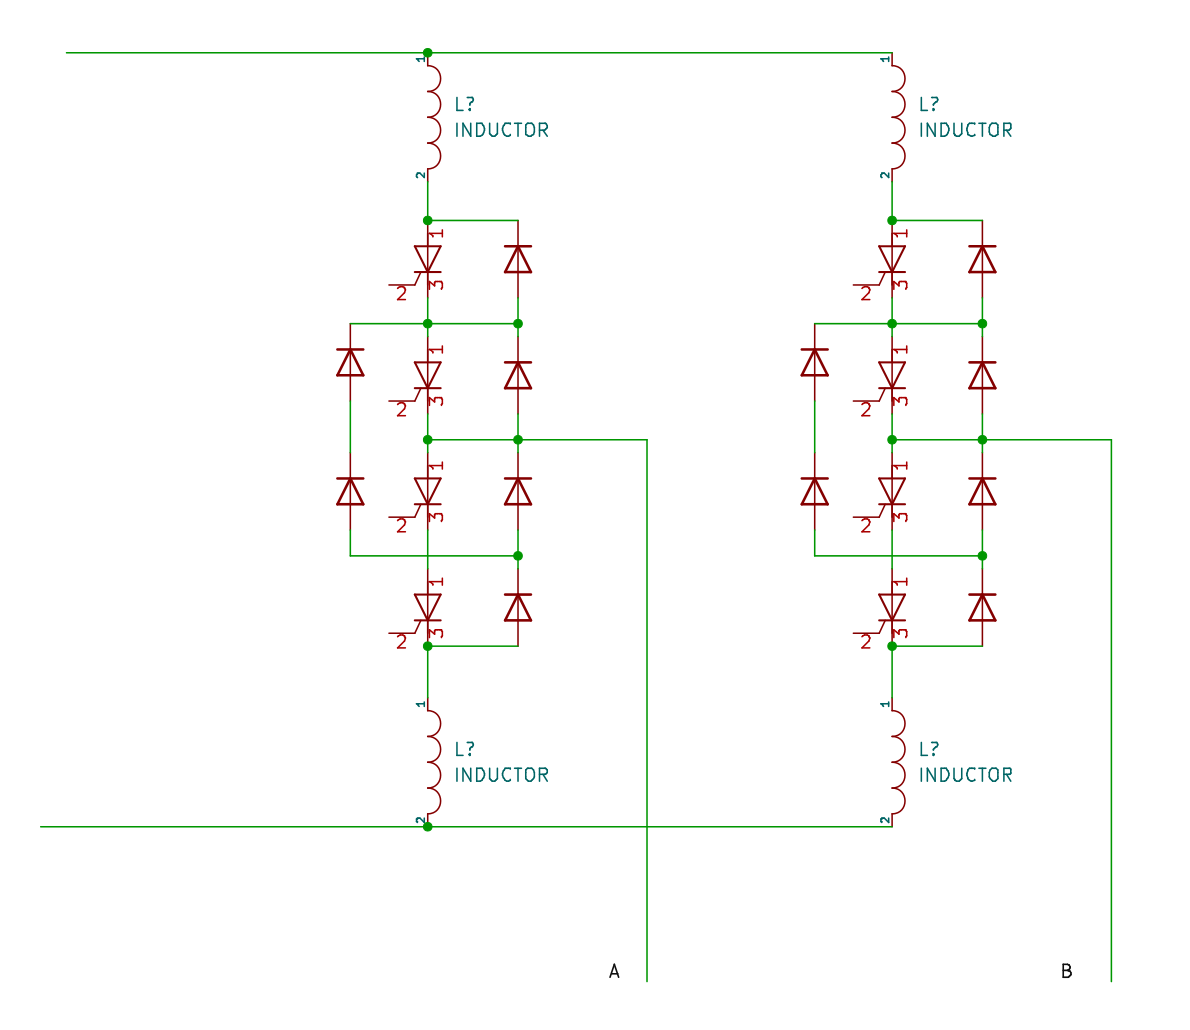
\includegraphics[width=\textwidth,frame]{Bilder/umrichter_schaltbild.png}
      \caption{3-Level 4QS}
    \end{minipage}
    \hfill
    \begin{minipage}[b]{0.4\textwidth}
        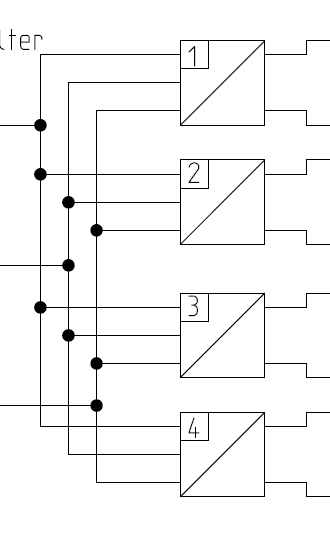
\includegraphics[width=\textwidth,frame]{Bilder/umrichter_16.png}
      \caption{Anschluss der Umrichter an Zwischenkreis und Summiertrafo}
    \end{minipage}
  \end{figure}
\clearpage

\subsection{Bemessungsdaten Umrichter 16.7 Hz}
\begin{table}[htb]
    \centering
    \caption[]{Umrichter 16.7 Hz}
    \begin{NiceTabular}{|l|p{4cm}|}[hvlines]
        \CodeBefore
        \columncolor{lightergray}{1}
        \Body
         Nennscheinleistung pro Umrichter& $\SI{5}{\unit{\mega\volt\ampere}}$\\
         Nennwirkleistung pro Umrichter& $\SI{4}{\unit{\mega\watt}}$\\
         Nenneingangsspannung DC  & $\SI{5000}{\V}$\\
         Nennausgangaspannung AC (RMS) & $\SI{3535}{\V}$\\
         Nennfrequenz AC-Seite  & $\SI{16.7}{\Hz}-6\%+4\%$\cite*{DeutschesInstitutfurNormungene.V..200802}\\
         Wirkungsgrad& $>95\%$\\  
         Nennstrom DC pro Umrichter & $\SI[]{1.4}[]{\kilo\ampere}$  \\
         max. Strombelastung Halbleiter (WS Seitig) & \SI[]{1714}[]{\A}\\ 
         max. Spannungsbelastung Halbleiter (WS Seitig)& \SI[]{1767}[]{\V}\\
         Sicherheitsfaktor $f_I$ & $1.65$\\
         Sicherheitsfaktor $f_u$ & $1.8$\\
    \end{NiceTabular}
\end{table}

\subsection{Bemessungsdaten Umrichter 50 Hz als Gleichrichter}
\begin{table}[htb]
    \centering
    \caption[]{Umrichter 50 Hz}
    \begin{NiceTabular}{|l|p{4cm}|}[hvlines]
        \CodeBefore
        \columncolor{lightergray}{1}
        \Body
         Nennwirkleistung pro Umrichter& $\SI{5.8}{\unit{\mega\watt}}$\\
         Nenneingangsspannung AC  & $\SI{3537}{\V}$\\
         Nennausgangaspannung DC & $\SI{5000}{\V}$\\
         Nennfrequenz AC-Seite  & $\SI{50}{\Hz}$\\
         Wirkungsgrad& $>95\%$\\  
         Nennstrom DC pro Umrichter & $\SI[]{1.667}[]{\kilo\ampere}$  \\
         max. Strombelastung Halbleiter (WS Seitig) & \SI[]{1714}[]{\A}\\ 
         max. Spannungsbelastung Halbleiter (WS Seitig)& \SI[]{1767}[]{\V}\\
         Sicherheitsfaktor $f_I$ & $1.65$\\
         Sicherheitsfaktor $f_u$ & $1.8$\\
    \end{NiceTabular}
\end{table}



\subsection{Funktionsprüfung}

\subsubsection*{Typrüfung}
\begin{itemize}[noitemsep]
    \item Sichtprüfung
    \item Überprüfung von Hilfsgeräten
    \item Isolationsprüfung 
    \item Überprüfung von Schutzeinrichtungen
    \item Schwachlast- und Funktionsprüfung
    \item Prüfung der Bemessungs-Ausgangsleistung
    \item Überstromprüfung
    \item Erwärmungsprüfung
    \item Bestimmung der Verlustleistung
    \item Messung der Ausgangsspannung
    \item Bestätigung des Einstellbereiches der Ausgangsspannung
    \item Bestätigung des Einstellbereiches der Ausgangsfrequenz
    \item Überprüfung der automatischen Steuerung und Regelung
\end{itemize}
\subsubsection*{Stückprüfung}
\begin{itemize}[noitemsep]
    \item Sichtprüfung
    \item Überprüfung von Hilfsgeräten
    \item Isolationsprüfung 
    \item Überprüfung von Schutzeinrichtungen
    \item Schwachlast- und Funktionsprüfung
    \item Messung der Ausgangsspannung
    \item Bestätigung des Einstellbereiches der Ausgangsspannung
\end{itemize}

\subsubsection*{Zusätzliche Prüfungen}
\begin{itemize}[noitemsep]
    \item Kurzschlussprüfung
    \item Messung hörbarer Geräusche
    \item Störfestigkeitsprüfung 
    \item Emissionsprüfung
    \item Messung der überlagerten Wechselspannung und des überlagerten Wechselstromes
\end{itemize}


\subsubsection*{Normen}
\begin{itemize}
    \item DIN EN 60146-2: Halbleiter-Stromrichter Teil 2: Selbstgeführte Halbleiter-Stromrichter
    einschließlich Gleichstrom-Direktumrichter
\end{itemize}
                                                           